\subsection{Formaldeide}

\subsubsection{Ottimizzazione geometrica e simmetria}

Abbiamo considerato la formaldeide in quanto essa risulta il composto
organico pi\`u semplice
per la trattazione \textit{ab initio} del gruppo carbonilico. 

Come punto di partenza per l'approccio computazionale si \`e fatto uso di
una geometria sperimentale, successivamente ottimizzata mediante il programma
\texttt{dalton}. La tabella \ref{tab:geom_formaldeide} mostra i parametri geometrici
caratteristici della formaldeide nello stato fondamentale, ottimizzati con
differenti metodi nella base 6-311G*

\begin{center}
\begin{threeparttable}
\caption{\small Formaldeide - geometrie di equilibrio}
\label{tab:geom_formaldeide}
\small
\begin{tabular}{|c|ccc|}
\hline
					& HF			& CAS			 	&  Exp.\tnote{1} \\
\hline
$r$(C-O)			&  1.1782		& 1.2161			&  1.2078 \\
$r$(C-H)			&  1.0936	 	& 1.0885 			&  1.1161 \\
$\angle$(H-C-H)		&  115.94 	 	& 117.20			&  116.50 \\
$\angle$(H-C-O)		&  122.03 	 	& 121.40			&  121.75 \\
Energia				&  1.895765 	& 1.968732			&         \\
\hline
\end{tabular}
\begin{tablenotes}
 \item[1] \small Cfr. \cite{jpsj-18-1963-1174} e \cite{jpc-97-17-1993-4293}
 \item[] \small Valori in Angstroms. Angoli in gradi. Energia come \mbox{-(112 + valore)} Hartree.

\end{tablenotes}
\end{threeparttable}
\end{center}

Possiamo notare come i risultati ottenuti a livello CASSCF siano in
migliore accordo con i valori sperimentali rispetto ai risultati ottenuti a
livello HF.
Il sistema appartiene al gruppo di simmetria C$_{2v}$, la cui tavola dei
caratteri \`e qui rappresentata

\begin{center}
\begin{tabular}{c|cccc|c|c}
  $C_{2v}$  & E &  $C_2$ & $\sigma_{xz}$ & $\sigma_{yz}$ &  &  \\
\hline
    $A_1$  &   1 &   1 &   1 &   1 & z & $x^2$, $y^2$, $z^2$ \\
    $B_1$  &   1 &  -1 &   1 &  -1 & x, $R_y$ & xz \\
    $B_2$  &   1 &  -1 &  -1 &   1 & y, $R_x$ & yz \\
    $A_2$  &   1 &   1 &  -1 &  -1 & $R_z$ & xy \\
\end{tabular}
\end{center}

La molecola \`e disposta sul piano $yz$, con l'asse C$_2$ colineare all'asse $z$.

Il calcolo CAS fa riferimento ad un sistema con 6 elettroni attivi in uno
spazio di 5 orbitali. La figura \ref{fig:formaldeide_orbitali} mostra
le forme degli orbitali e le rispettive simmetrie.
\begin{figure}[htb]
\begin{center}
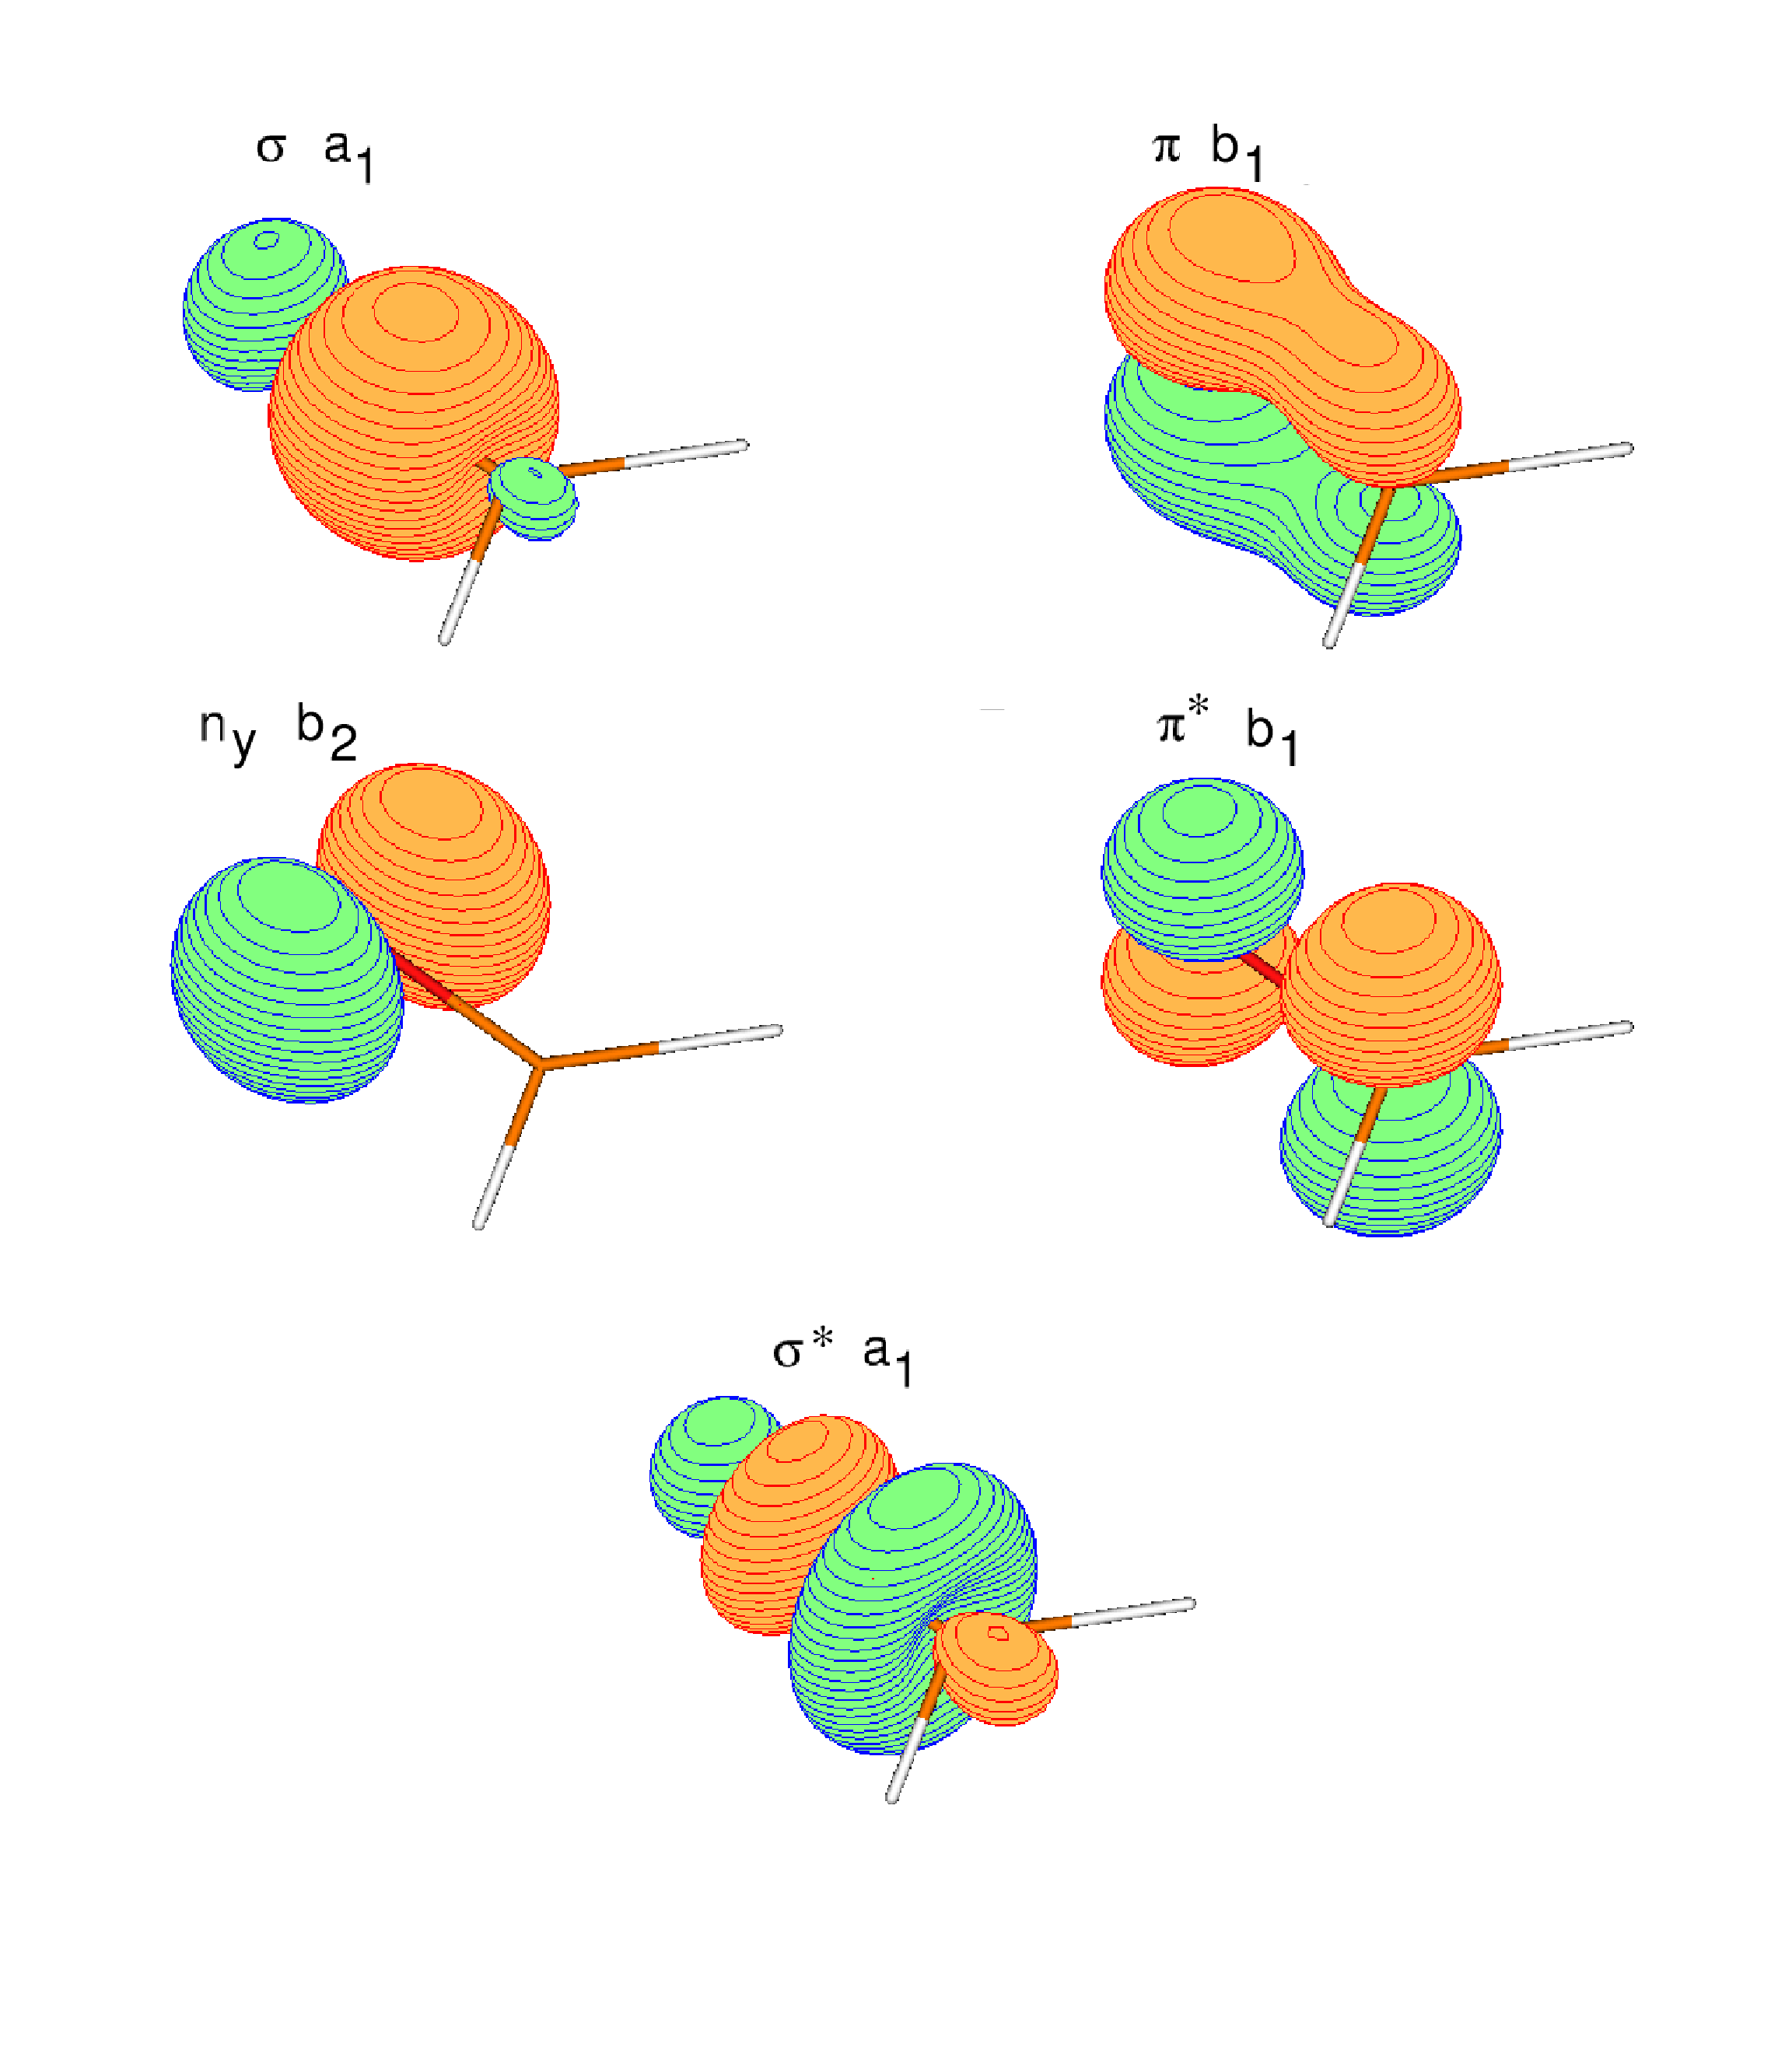
\includegraphics[width=8cm,keepaspectratio]{immagini/formaldeide/orbitali.eps}
\end{center}
\caption{Spazio CAS per la formaldeide}
\label{fig:formaldeide_orbitali}
\end{figure}

Nella trattazione HF gli orbitali doppiamente occupati sono
\begin{itemize}
\item 5 di simmetria A$_1$
\item 1 di simmetria B$_1$
\item 2 di simmetria B$_2$
\end{itemize}
Lo spazio CAS \`e stato costruito utilizzando, per lo spazio di core
(doppiamente occupato) 4 orbitali A$_1$ e 1 orbitale B$_2$,
mentre lo spazio attivo \`e stato definito da 2 orbitali A$_1$
(l'orbitale legante $\sigma$ e l'antilegante $\sigma^{*}$), 2 orbitali B$_1$
(un legante $\pi$ e l'antilegante $\pistar$) e 1 orbitale B$_2$ (non legante 
$n_y$), con 6 elettroni attivi e 10 elettroni di core.
Con questa scelta, sono necessarie 18 configurazioni per descrivere la molecola
nello stato fondamentale (simmetria A$_1$). 

Nel caso della transizione elettronica di interesse, si avr\`a la promozione
di un elettrone dall'orbitale $n_y$, di simmetria B$_2$, all'orbitale $\pistar$,
di simmetria B$_1$. La tabella dei prodotti diretti delle rappresentazioni
per il gruppo C$_{2v}$ 
\begin{center}
\begin{tabular}{|c|cccc|}
\hline
 C$_{2v}$ & A$_1$ & B$_1$ & B$_2$ & A$_2$ \\
\hline                                
    A$_1$ & A$_1$ &       &       &        \\
    B$_1$ & B$_1$ & A$_1$ &       &        \\
    B$_2$ & B$_2$ & A$_2$ & A$_1$ &        \\
    A$_2$ & A$_2$ & B$_2$ & B$_1$ & A$_1$  \\
\hline
\end{tabular}
\end{center}
indica per lo stato elettronico finale la simmetria B$_2 \otimes $B$_1 = $A$_2 $.

Il calcolo ha fornito, per lo spazio attivo del ground state, i seguenti numeri
di occupazione
\begin{verbatim}
 Simmetria A1 : 1.978929123   0.021519393
 Simmetria B1 : 1.929961079   0.070506119
 Simmetria B2 : 1.999084286
\end{verbatim}

L'energia CASSCF finale \`e -113.968732 Hartree, che si assume come energia
del ground state per il calcolo della transizione sulla base 6-311G*
a livello CASSCF.

%Limitatamente alla molecola di formaldeide sono state inoltre calcolate le
%energie di eccitazione per le transizioni $n_z \rightarrow \pistar$ e $\pi \rightarrow
%\pistar$, che comportano uno stato elettronico finale di simmetria $A_1 \otimes B_1 = B_1$
%e $B_1 \otimes B_1 = A_1$ rispettivamente. Di conseguenza, nel caso della
%transizione $\pi \rightarrow \pistar$, non avviene cambiamento di simmetria, dal momento
%che il ground state \`e anch'esso di simmetria $A_1$. L'energia dello stato eccitato
%sar\`a quindi la seconda radice della diagonalizzazione nella simmetria del ground state.

%In tabella \ref{tab:formaldeide_vertical} riportiamo i valori ottenuti per le varie transizioni,
%affiancate al dato sperimentale
%\begin{center}
%\begin{threeparttable}
%\caption{Formaldeide - energie di transizione verticale CAS/6-311G*}
%\label{tab:formaldeide_vertical}
%\small
%\begin{tabular}{|ccccc|}
%\hline
%							& Simm.		& Energia\tnote{1}	& Eccitato - GS\tnote{2} & Sperim.\tnote{2} \\
%\hline
%$GS$ 						& A1		& 1.96873 			& 0		& 0   \\
%$n_y \rightarrow \pistar$ 	& A2		& 1.80577 			& 4.43  & 4.07 \\
%$n_z \rightarrow \pistar$ 	& B1		& 1.59497			& 10.17 & 9.97 \tnote{3} \\
%$\pi \rightarrow \pistar$   & A1        & 1.55132           & 11.36 & 9.19 \tnote{3} \\
%\hline
%\end{tabular}
%\begin{tablenotes}
%\tiny
% \item[1] Energia come - (112 + valore) Hartree.
% \item[2] Valore in eV
% \item[3] Valore sperimentale non disponibile. Dati da CIS-MP2 su 6-311(2+,2+)G** (Cfr. \cite{jpc-97-17-1993-4293})
%\end{tablenotes}
%\end{threeparttable}
%\end{center}

Il calcolo effettuato sullo stato eccitato di simmetria A$_2$, mantenendo la
geometria ottimizzata per lo stato fondamentale (transizione verticale) ha fornito
invece un'energia di -113.80577 Hartree, comportando di conseguenza un'energia di
transizione elettronica pari a 4.43 eV, che confrontato al valore sperimentale
4.07 eV (Cfr. \cite{jpc-99-20-1995-8050}) evidenzia un errore di circa 0.4 eV. 
%Le altre transizioni non sono esattamente
%definite, e non vi sono ancora riferimenti bibliografici certi sull'assegnazione energetica
%della transizione $\pi \rightarrow \pistar$, che dovrebbe giacere tra i 9 e gli 11 eV. (Cfr.
%\cite{jpc-99-20-1995-8050}). Per questa ragione, tali calcoli non verranno affrontati su molecole
%pi\`u complesse, ma limiteremo il nostro studio alla sola transizione verticale e adiabatica
%$n_y \rightarrow \pistar$.

I numeri di occupazione confermano la transizione $n_y \rightarrow \pistar$
\begin{verbatim}
 Simmetria A1 : 1.984641659   0.015707156
 Simmetria B1 : 1.996255549   1.003395636
 Simmetria B2 : 1.000000000
\end{verbatim}

\`E stata successivamente condotta un'ottimizzazione di geometria per lo
stato eccitato, valutando di conseguenza la transizione adiabatica. In tali
condizioni, la simmetria del sistema cala da C$_{2v}$ a C$_s$, venendo a
mancare un piano di riflessione in seguito alla piramidalizzazione della
molecola.

\begin{center}
\begin{threeparttable}
\caption{\small Formaldeide - geometrie di transizione adiabatica}
\label{tab:formaldeide_geometrie_adiab}
\begin{tabular}{|c|cc|}
\hline
					& GS		& $n_y \rightarrow \pistar$ \\ %& $n_z \rightarrow \pistar$	\\
\hline
$r$(C-O)		 	& 1.2161	&  1.3817 				\\ %& 1.541100 					 \\
$r$(C-H)			& 1.0885	&  1.0762					\\ %& 1.078499					 \\
$\angle$(H-C-H)		& 117.20	&  119.44					\\ %& 115.812					 \\
$\angle$(H-C-O)		& 121.40	&  113.03					\\ %& 110.473					 \\
Energia 			& 1.968732	&  1.834522					\\ %& 1.673067					 \\
En. Eccitazione 	& 			&  3.65						\\ %& 8.04						 \\
En. Ecc. Exp.\tnote{1} & 	&  3.50						\\ %& 8.49						 \\
\hline
\end{tabular}
\begin{tablenotes}
\small
 \item[1] Cfr. \cite{sa-34a-1978-749} e \cite{jpc-97-17-1993-4293}
 \item[] Valori in Angstroms, angoli in gradi, Energie assolute come
  \mbox{-(112 + valore)} Hartree, energie di eccitazione in eV
\end{tablenotes}
\end{threeparttable}
\end{center}

La geometria da planare muta in piramidale. \`E osservabile uno spostamento
degli atomi di idrogeno fuori dal piano molecolare ed un allungamento del
legame C-O dovuto all'occupazione di un orbitale di antilegame $\pistar$,
accompagnato da una netta diminuzione dell'angolo di legame H-C-O verso
valori caratteristici di una geometria piramidale.

A causa del calo di simmetria del sistema, gli orbitali precedentemente
riconducibili alle rappresentazioni A$_1$ e B$_1$ appartengono ora alla
rappresentazione A$^{\prime}$, mentre gli orbitali appartenenti alle 
rappresentazioni B$_2$ e A$_2$ ora saranno di simmetria A$^{\prime\prime}$.
Lo spazio attivo precedentemente definito vedr\`a di conseguenza, 
$\sigma$, $\sigma^{*}$, $\pi$ e $\pistar$ appartenere ad A$^{\prime}$,
e $n_y$ ad A$^{\prime\prime}$. Una transizione elettronica $n_y \rightarrow
\pistar$ avr\`a simmetria A$^{\prime\prime} \otimes $A$^{\prime} =
$A$^{\prime\prime}$

Lo stato eccitato ha un'energia CASSCF pari a -113.834522
Hartree, che comporta un'energia di transizione di 3.65 eV, contro un valore
sperimentale di 3.50 eV (Cfr. \cite{jpc-97-17-1993-4293} e \cite{sa-34a-1978-749})

\subsubsection{Dipendenza dalla base atomica}

Per valutare la dipendenza dalla base atomica utilizzata si sono effettuati calcoli per
le transizioni verticale e adiabatica $ n_y \rightarrow \pistar $ su differenti 
set di base, in ordine di dimensionalit\`a:
\begin{itemize}
 \item 6-31G (Cfr. \cite{mp-27-1974-209})
 \item cc-pVDZ (Cfr. \cite{jcp-90-1989-1007})
 \item ano-1 (Cfr. \cite{jcp-55-1971-4798}) con riduzione 3s2p1d per il carbonio e 2s1p per l'idrogeno
 \item 6-311G* (Cfr. \cite{jcp-72-1980-5639})
 \item cc-pVTZ (Cfr. \cite{jcp-90-1989-1007})
 \item cc-pVQZ (Cfr. \cite{jcp-90-1989-1007})
\end{itemize}
Su ogni base \`e stata effettuata una ottimizzazione di geometria della
molecola, a livello CASSCF.

La tabella \ref{tab:formaldeide_vertical_basis} riporta i risultati ottenuti
per la transizione verticale. \`E evidente come basi a dimensionalit\`a molto
elevata, come cc-pVTZ e cc-pVQZ, portino a risultati pressoch\'e identici.
\`E quindi prevedibile che una ulteriore estensione della base non fornirebbe
risultati pi\`u accurati di quelli ottenuti, e comporterebbe un notevole incremento
dei tempi di calcolo. L'errore commesso a livello CASSCF resta
considerevole, essendo di 0.34 eV.  Una possibile soluzione alternativa \`e
ricercabile nell'allargamento dello spazio CAS, che aumenterebbe in modo
deciso la complessit\`a computazionale.

Di conseguenza, per cercare di migliorare i risultati CASSCF abbiamo
condotto dei calcoli perturbativi utilizzando la teoria NEV-PT, ottenendo
ottimi risultati con tempi di calcolo pi\`u che accettabili. La
tabella \ref{tab:formaldeide_vertical_basis} mostra quanto ottenuto, sia per
l'approccio Strongly Contracted (NEV-PT/SC) che per quello Partially Contracted
(NEV-PT/PC).

\begin{center}
\begin{threeparttable}
\caption{\small Formaldeide - Energia di transizione $n_y \rightarrow \pistar$ verticale di singoletto, metodi CASSCF e CASSCF/NEV-PT}
\label{tab:formaldeide_vertical_basis}
{
\small
\begin{tabular}{|c|ccc|ccc|}
\hline
 Base	& \multicolumn{3}{c}{GS\tnote{1}}				& \multicolumn{3}{c|}{$n_y \rightarrow \pistar$ vert.\tnote{2}} \\
		& CASSCF		& NEV-PT & NEV-PT	& CASSCF		& NEV-PT & NEV-PT \\
		& 				& SC	 & PC		& 				& SC 	& PC \\
\hline
6-31G	& 1.891188		& 2.019821		& 2.021959		& 3.85			& 3.73		& 3.72		    \\
cc-pVDZ	& 1.950044		& 2.183100		& 2.185533		& 4.38			& 4.07 		& 4.10			\\
ano-1	& 1.978883		& 2.207808		& 2.210750		& 4.36			& 4.02 		& 4.01			\\
6-311G*	& 1.968732		& 2.242321		& 2.244788		& 4.43 			& 4.07		& 4.11 			\\
cc-pVTZ & 1.985284 		& 2.316323		& 2.319135		& 4.40			& 4.04 		& 4.02			\\
cc-pVQZ & 1.994326		& 2.381916		& 2.384828		& 4.41			& 4.04		& 4.02			\\
\hline
\hline
Exp.	&				& 				&				& \multicolumn{3}{c|}{4.07} \\
\hline
\end{tabular}
}
\begin{tablenotes}
\small
 \item[1] Energia come -(112 + valore) Hartree
 \item[2] Valori in eV
\end{tablenotes}
\end{threeparttable}
\end{center}

Per quanto riguarda la transizione adiabatica, si \`e tenuto conto della differenza
tra le energie di punto zero (Zero Point Energy, ZPE) dei due stati elettronici. Questa differenza deriva
dalla diversa struttura della superficie di potenziale per lo stato fondamentale ed
eccitato, che si riflette in una diversa energia dello stato vibrazionale
fondamentale per i due stati elettronici. Assumendo che l'effetto perturbativo non attui modifiche
significative sulla struttura del potenziale CASSCF, ma si limiti ad una
traslazione energetica omogenea, le energie di punto zero per i calcoli
perturbativi possono essere assunte uguali a quella CASSCF. 
Ci\`o non \`e strettamente garantito, tuttavia \`e una approssimazione necessaria,
in quanto una accurata valutazione di questo effetto necessiterebbe di un
calcolo accurato di tutta la superficie di potenziale a livello
perturbativo.
Per questa ragione, la correzione ZPE
\`e stata applicata allo stesso modo sia sul calcolo CASSCF che sul calcolo 
perturbativo.

\begin{center}
\begin{threeparttable}
\caption{\small Formaldeide - Energia di transizione $n_y \rightarrow \pistar$ adiabatica di singoletto, calcolata a livello CASSCF e NEV-PT}
\label{tab:formaldeide_basis_energy}
{
\small
\begin{tabular}{|c|cccccc|}
\hline
Base	& ZPE 			& ZPE 				& $\Delta$ZPE	& CASSCF	& NEV-PT	& NEV-PT \\
		& (GS)			& (Ecc.)			& 				& ZPE 		&   SC/ZPE 	& PC/ZPE \\
\hline
6-31G	& 0.766			& 0.685				& -0.081		&  3.13		& 3.12			  & 3.14			\\
cc-pVDZ & 0.760			& 0.692				& -0.068        &  3.56		& 3.49			  & 3.50			\\
ano-1	& 0.764			& 0.696				& -0.068		&  3.55		& 3.43			  & 3.45			\\
6-311G* & 0.765			& 0.700				& -0.066		&  3.59		& 3.52			  & 3.57			\\
cc-pVTZ & 0.759         & 0.692				& -0.067		&  3.60		& 3.55			  & 3.56			\\
cc-pVQZ & 0.760			& 0.693				& -0.067		&  3.61		& 3.58			  & 3.59			\\
\hline
\hline
Exp.	&				& 					& 				& \multicolumn{3}{c|}{3.50}						\\
\hline
\end{tabular}
}
\begin{tablenotes}
\small
 \item[ ] Valori in eV
\end{tablenotes}
\end{threeparttable}
\end{center}

In figura \ref{fig:formaldeide_gs} sono rappresentate le energie elettroniche del
ground state a livello CASSCF (linea rossa), NEV-PT/SC (linea verde) e
NEV-PT/PC (linea blu), in funzione della base atomica scelta, in ordine di
dimensionalit\`a. Come si pu\`o notare, la NEV-PT/SC fornisce
risultati di pochissimo superiori in energia alla NEV-PT/PC.

\begin{figure}[ht]
\begin{center}
\includegraphics[angle=270,width=10cm,keepaspectratio]{immagini/formaldeide/gs.eps}
\parbox[h]{10cm}{
\caption{\small Formaldeide - Energia dello stato fondamentale a livello CASSCF (linea rossa),
NEV-PT/SC (linea verde) e NEV-PT/PC (linea blu). }
\label{fig:formaldeide_gs}
}
\end{center}
\end{figure}
\clearpage

Analogamente, le figure \ref{fig:formaldeide_vert} e
\ref{fig:formaldeide_adiab} forniscono la medesima rappresentazione
relativamente agli stati eccitati calcolati alla geometria di equilibrio
dello stato fondamentale e dello stato eccitato rispettivamente. 

\begin{figure}[ht]
\begin{center}
\includegraphics[angle=270,width=7cm,keepaspectratio]{immagini/formaldeide/vert.eps}
\parbox[h]{12cm}{
\caption{\small Formaldeide - Energia dello stato eccitato (transizione verticale)
a livello CASSCF (linea rossa), NEV-PT/SC (linea verde) e NEV-PT/PC (linea blu) come
funzione della base atomica. }
\label{fig:formaldeide_vert}
}
\end{center}
\end{figure}
\begin{figure}[ht]
\begin{center}
\includegraphics[angle=270,width=7cm,keepaspectratio]{immagini/formaldeide/adiab.eps}
\parbox[h]{12cm}{
\caption{\small Formaldeide - Energia dello stato eccitato (transizione
adiabatica) a livello CASSCF (linea rossa), NEV-PT/SC (linea verde) e NEV-PT/PC (linea blu) come
funzione della base atomica. }
\label{fig:formaldeide_adiab}
}
\end{center}
\end{figure}
\clearpage

Diagrammando l'energia della transizione verticale contro la base, si ottiene
il grafico in figura \ref{fig:formaldeide_energie_vert}. La simbologia
utilizzata \`e analoga a quella della figura precedente. La linea viola denota
il valore sperimentale di $4.07$ eV.

\begin{figure}[ht]
\begin{center}
\includegraphics[angle=270,width=12cm,keepaspectratio]{immagini/formaldeide/energie_vert.eps}
\parbox[h]{12cm}{
\caption{\small Formaldeide - energia di transizione verticale su basi differenti a livello CASSCF (linea rossa), NEV-PT/SC (linea verde) e NEV-PT/PC (linea blu) come funzione della base atomica.}
\label{fig:formaldeide_energie_vert}
}
\end{center}
\end{figure}

\`E possibile vedere come la transizione verticale venga descritta con buona accuratezza
anche con basi piccole, una volta che si sia introdotta la correzione perturbativa.
\clearpage

L'energia della transizione adiabatica in figura
\ref{fig:formaldeide_energie_adiab} mostra invece l'andamento di tale
parametro contro il valore sperimentale di $3.50$ eV.

\begin{figure}[ht]
\begin{center}
\includegraphics[angle=270,width=12cm,keepaspectratio]{immagini/formaldeide/energie_adiab.eps}
\parbox[h]{12cm}{
\caption{\small Formaldeide - energia di transizione adiabatica su basi differenti a livello CASSCF (linea rossa), NEV-PT/SC (linea verde) e NEV-PT/PC (linea blu) come funzione della base atomica.}
\label{fig:formaldeide_energie_adiab}
}
\end{center}
\end{figure}

\clearpage

%%%%%%%%%%%%%%%%%%%%%%%%%%%%%%%%%%%%%%%%%%%%%%%
